\documentclass{beamer}

\usepackage{fontspec}
\usepackage{xeCJK}
\setCJKmainfont[BoldFont=Noto Serif CJK TC Bold]{Noto Serif CJK TC}
\XeTeXlinebreaklocale "zh"
\XeTeXlinebreakskip = 0pt plus 1pt
\linespread{1.3}
\allowdisplaybreaks

\usepackage{color}
\usepackage{booktabs}
\usepackage{tabularx}
\usepackage{caption}
\usepackage{tikz}
\usepackage{verbatim}
\usepackage{pgfplotstable}
\pgfplotsset{width=12cm}
\pgfplotsset{height=7cm}
\pgfplotsset{compat=1.13}

\usetheme{EastLansing}
\usetikzlibrary{positioning}
\useinnertheme{rectangles}
\usefonttheme{professionalfonts}

\newcommand{\lw}{0.8mm}
\setbeamercovered{transparent}


%\AtBeginSection[]
%{
  %\begin{frame}<beamer>
	%\frametitle{報告大綱}
	%%\frametitle{RoadMap}
    %\tableofcontents[currentsection]
  %\end{frame}
%}

\title{Paper Intro}
\subtitle{\textcolor[rgb]{0.00,0.50,1.00}{{Speech Processing \& Machine Learning Laboratory}}}
\author{徐瑞陽}
\date{2020/02/20}
\begin{document}

\begin{frame}
\maketitle
\end{frame}



\begin{frame}
\frametitle{Outline}
\tableofcontents
\end{frame}

\section{Meta-Learning with Implicit Gradients}
\begin{frame}
  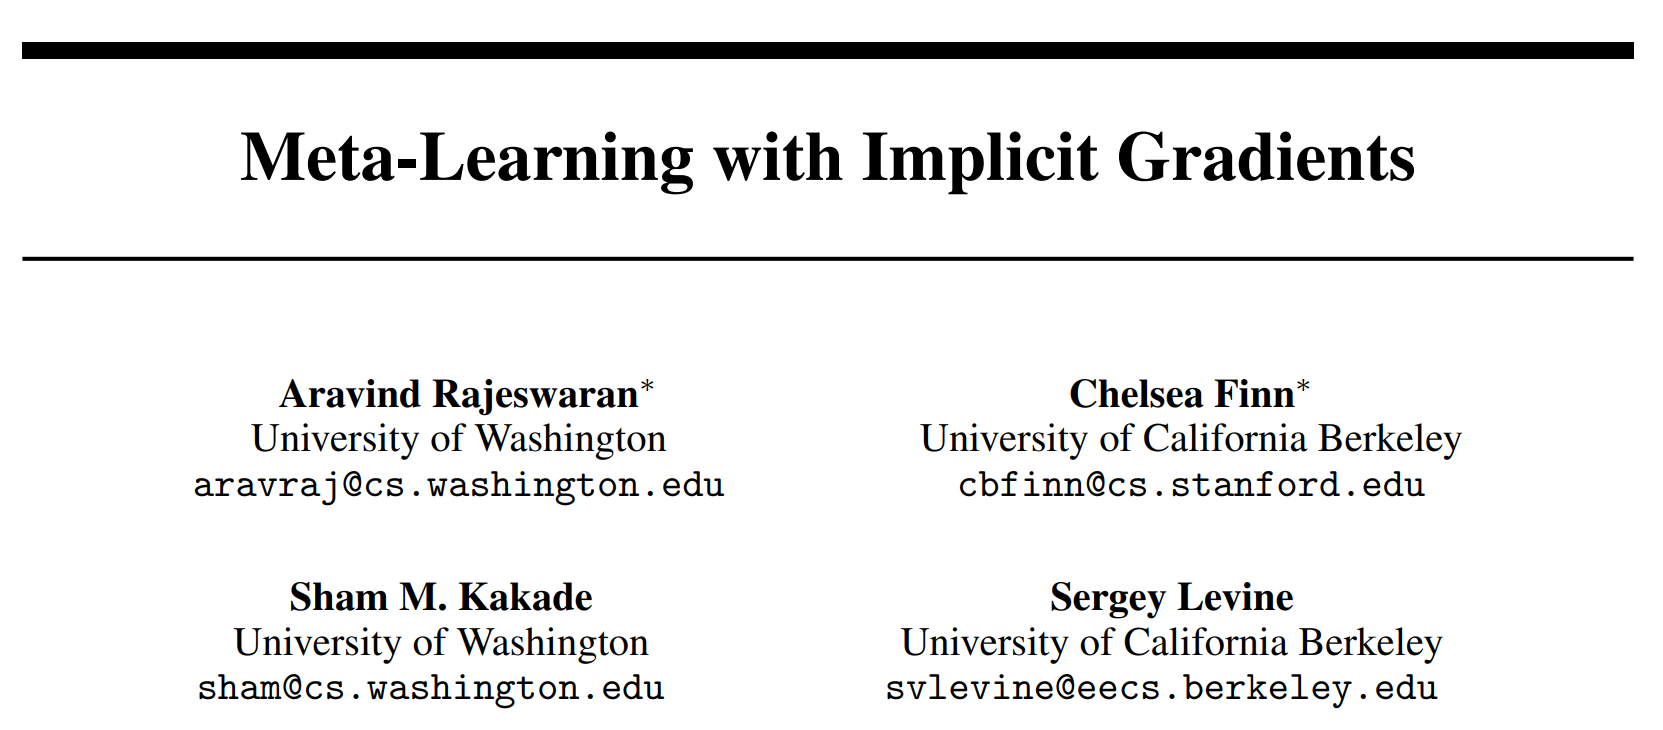
\includegraphics[width=\textwidth]{fig/iMAML-title.png}
  \center NeurIPS 2019
\end{frame}

\begin{frame}{Motivation: Challenge of MAML}
  When calculating meta-gradient, the computation cost (time/memory) is linearly growing with the inner update steps takes \\  (i.e related to the path length)

  \pause

  Can we obtain meta-gradient only from the adapted parameters\\ (i.e the last step)
\end{frame}

\begin{frame}[t]{Illustration: Gradient Calculation}
  \center 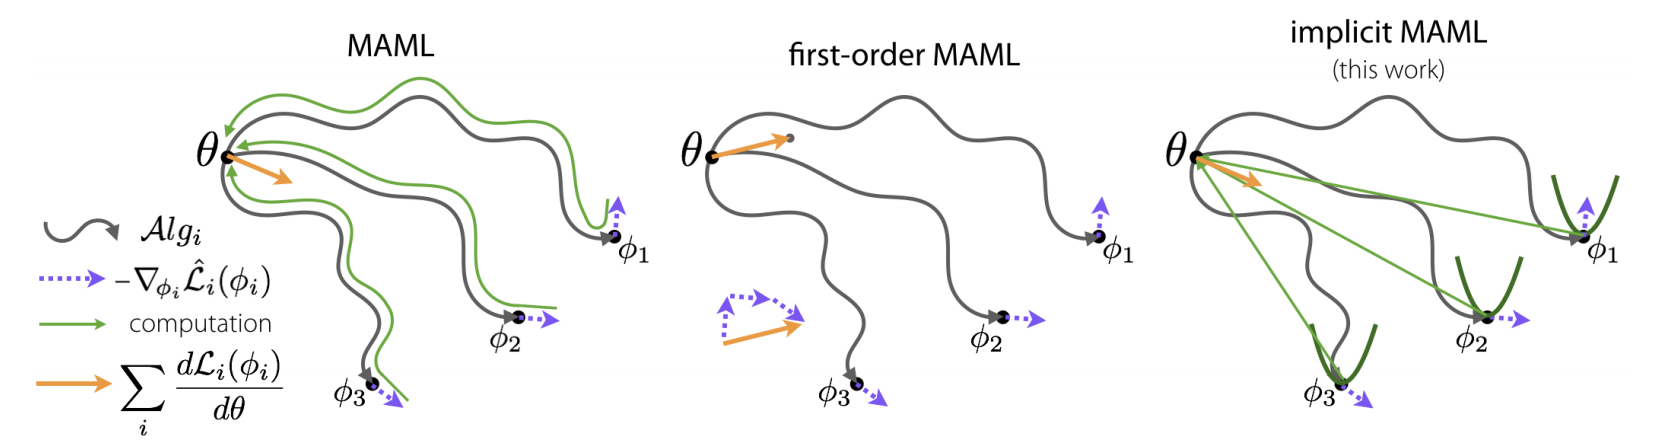
\includegraphics[width=\textwidth]{fig/iMAML-illustraion.png}
\end{frame}

\begin{frame}[t]{MAML in detail}
  Notation:
  \begin{itemize}
    \item init param: $\theta$
    \item dataset for task $i$: $D^{tr}_i$
    \item adapted param on $D^{tr}_i$: $\phi_i$
  \end{itemize}

  In inner loop (1-step GD for example)

  \begin{equation*}
    \phi_i = \mathcal{A}(\theta, D^{tr}_i) = \theta - \alpha \nabla_\theta \mathcal{L}^{tr}_i(\theta)
  \end{equation*}

\end{frame}

\begin{frame}[t]{MAML in detail}
  Meta Objective

  \begin{equation*}
    F(\theta) = \sum_i \mathcal{L}^{test}_i(\phi_i)
  \end{equation*}

  Meta gradient in one task:

  \begin{equation*}
    \frac{d \mathcal{L}^{test}_i(\phi_i)}{d \theta} = \nabla_\phi L^{test}_i (\phi) \cdot \frac{d \phi}{d \theta}
  \end{equation*}
\end{frame}

\begin{frame}[t]{MAML in detail: more GD steps}
  \center 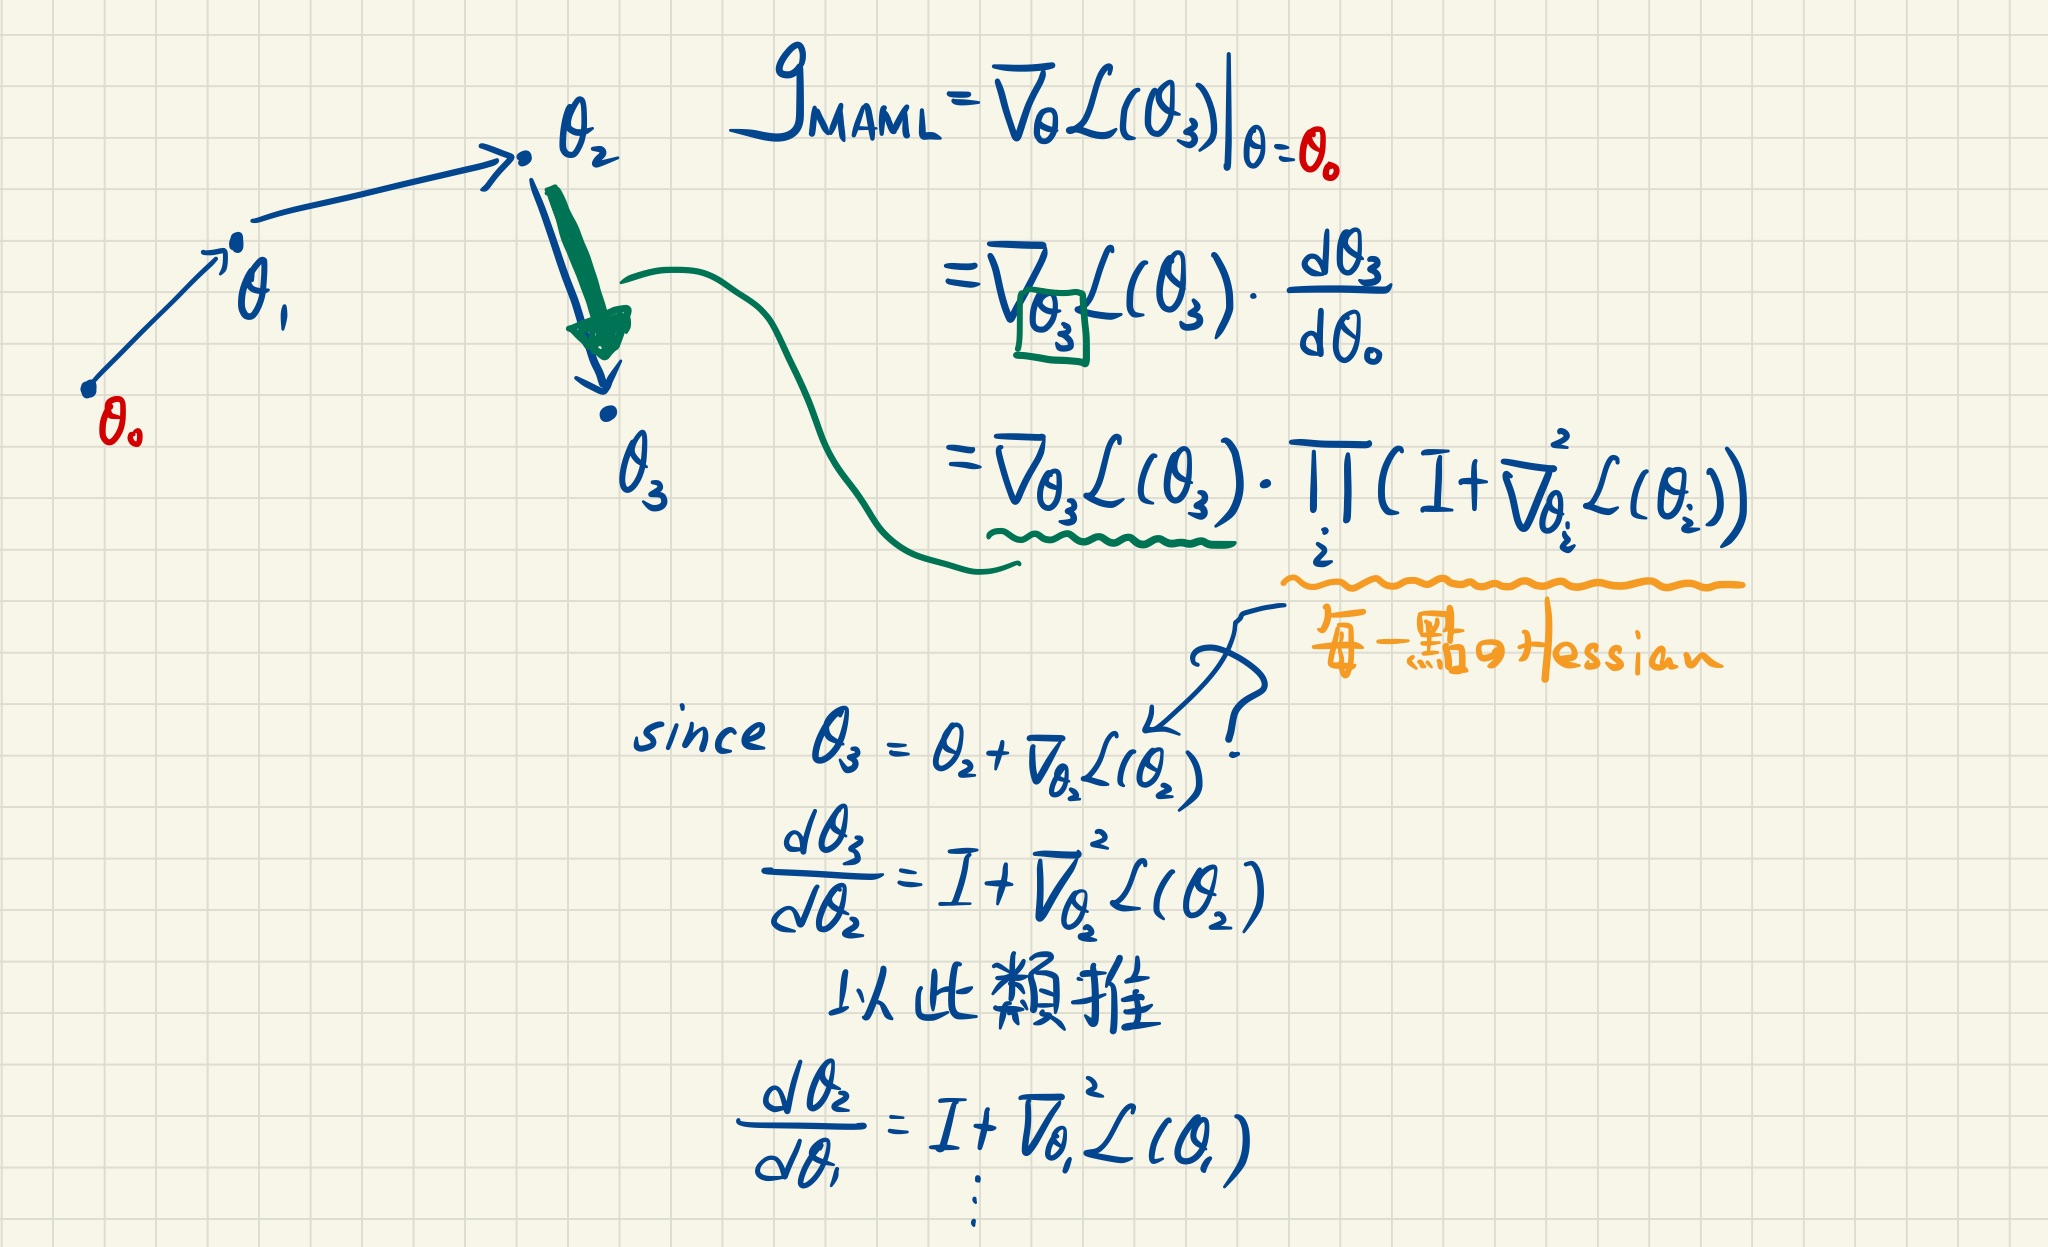
\includegraphics[width=\textwidth]{fig/iMAML-more-step.png}
\end{frame}

\begin{frame}[t]{Idea of iMAML}
  Incorporate proximal (鄰近的) regularization (explicit gaussian prior here)

  Meta objective for one task:

  \begin{equation*}
    \boxed{\mathcal{L}_{\text{new}}(\phi_i) = \mathcal{L}^{test}_i(\phi_i) + ||\phi_i - \theta||^2}
  \end{equation*}
\end{frame}

\begin{frame}[t]{Meta gradient of iMAML}
  What is $\frac{d \phi_i}{d \theta}$ ?

  Use implicit differentiation to solve !
  \center 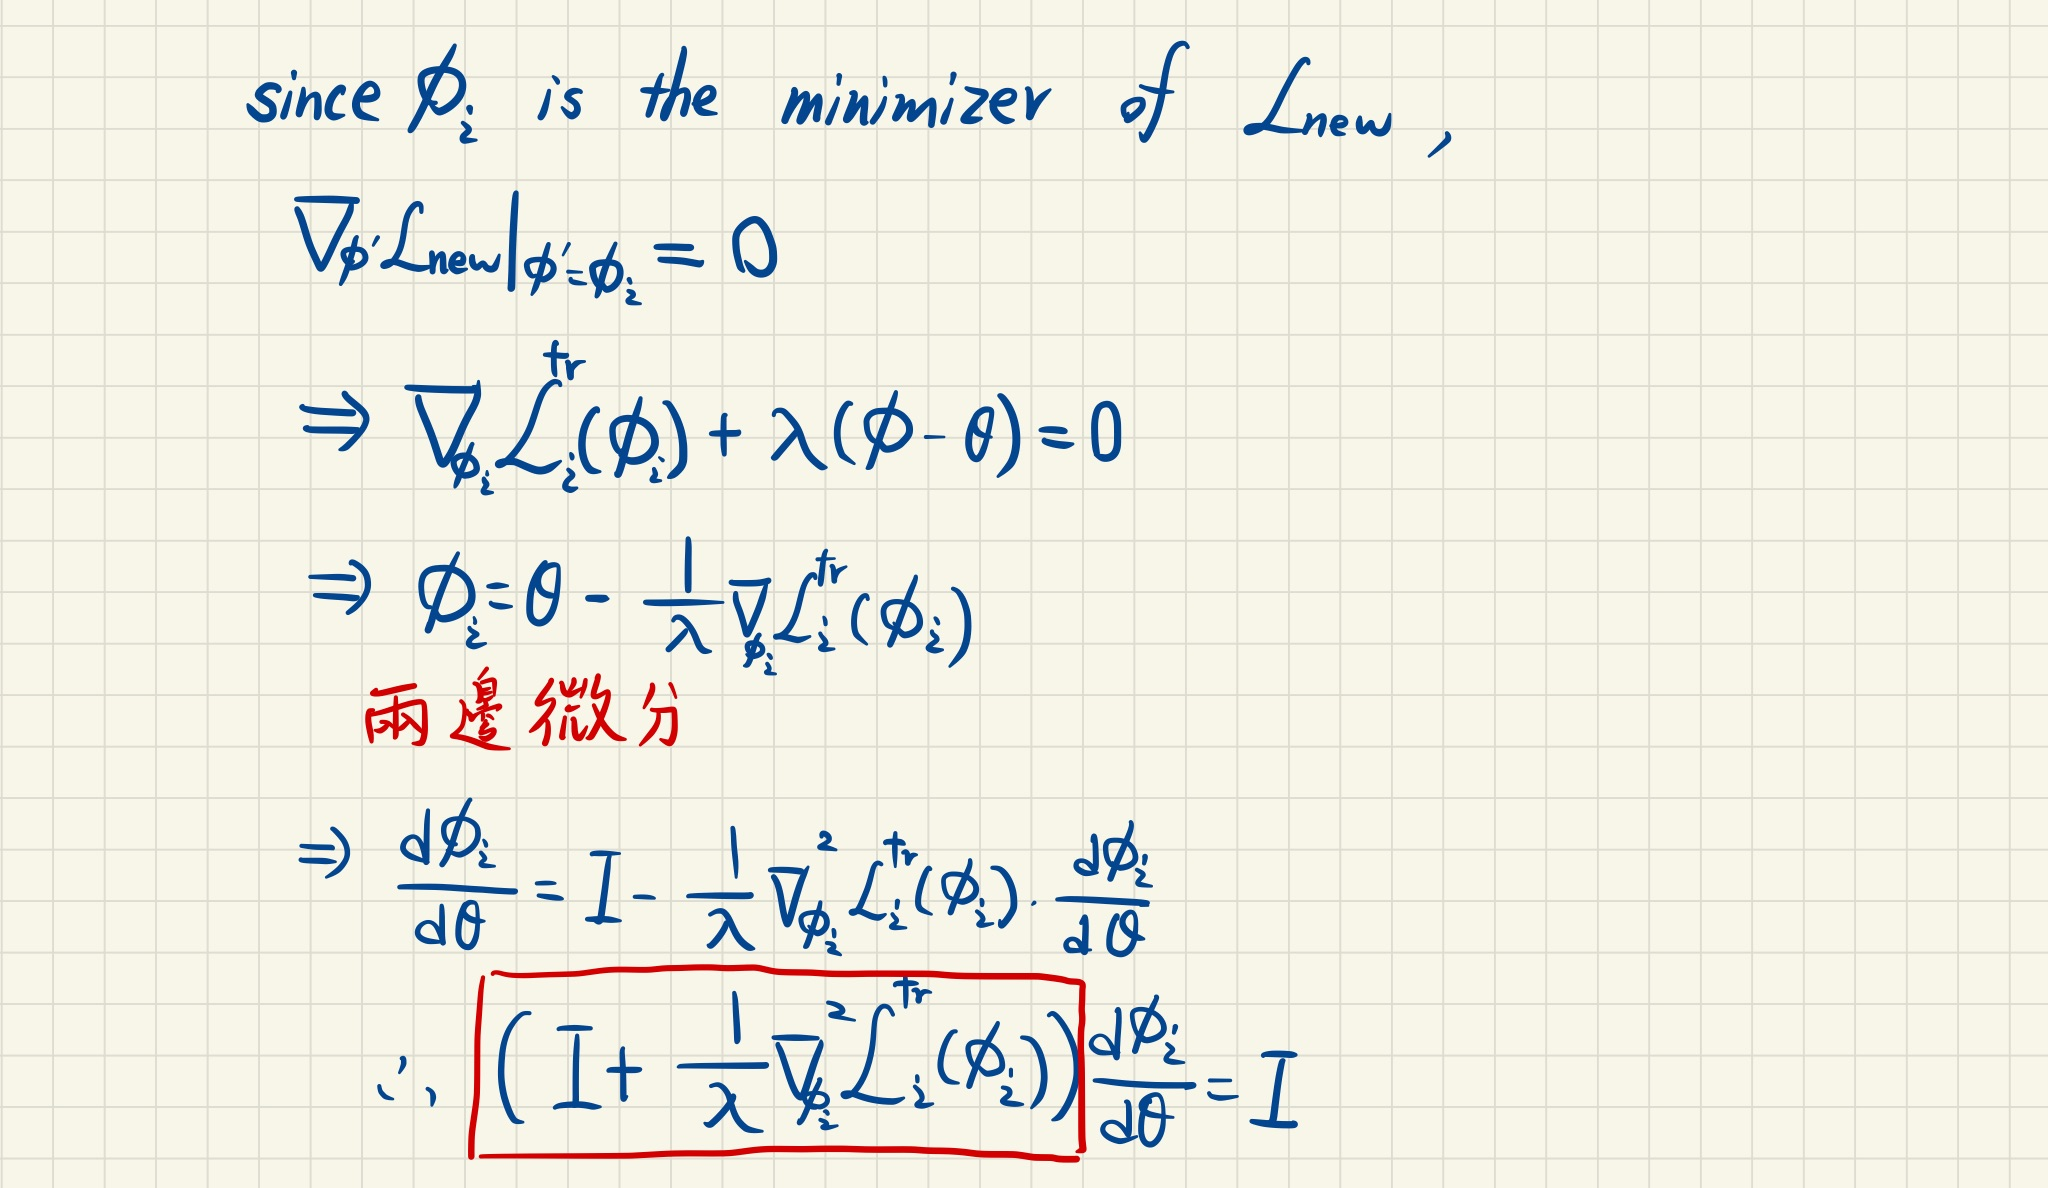
\includegraphics[width=0.8\textwidth]{fig/iMAML-grad.png}
\end{frame}

\begin{frame}[t]{$\delta$-approximate Hessian-vector product}
  \begin{equation*}
    ||w - A^{-1}b|| \leq \delta
  \end{equation*}

  \begin{equation*}
    \boxed{ w^\star = \arg\min_w w^T A w - w^T b }
  \end{equation*}

  \begin{itemize}
    \item $A$ should be positive definiete
    \item $A = (I + \frac{1}{\lambda}\nabla^2_\phi\mathcal{L}^{train}_i(\phi_i))^{-1}$
    \item $b = \nabla_\phi \mathcal{L}^{test}_i(\phi_i)$
    \item $w$: meta-gradient
    \item Use \textbf{conjugate gradient} to iteratively solve!
  \end{itemize}
\end{frame}

\begin{frame}[t]{Memory/Time Requirement on 20W5S Omniglot}
  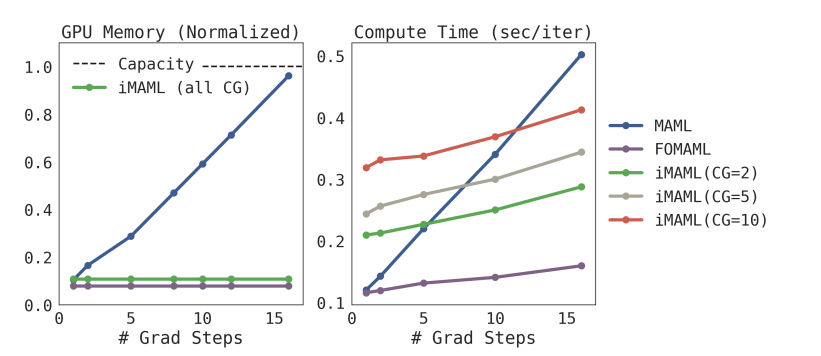
\includegraphics[width=\textwidth]{fig/iMAML-mt.png}
\end{frame}


\begin{frame}{Results on Omniglot}
  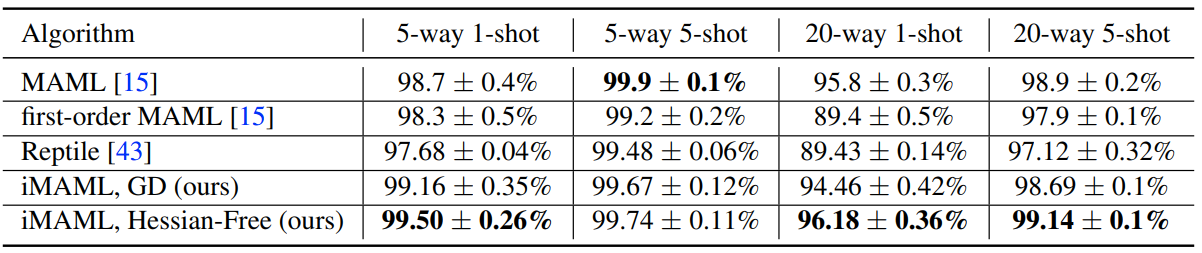
\includegraphics[width=\textwidth]{fig/iMAML-result.png}
Hessian-free: replace inner loop GD with Newton-CG
\end{frame}

\section{Meta Learning with Differentiable Closed-Form Solver}
\begin{frame}[t]{Meta Learning with Differentiable Closed-Form Solver}
  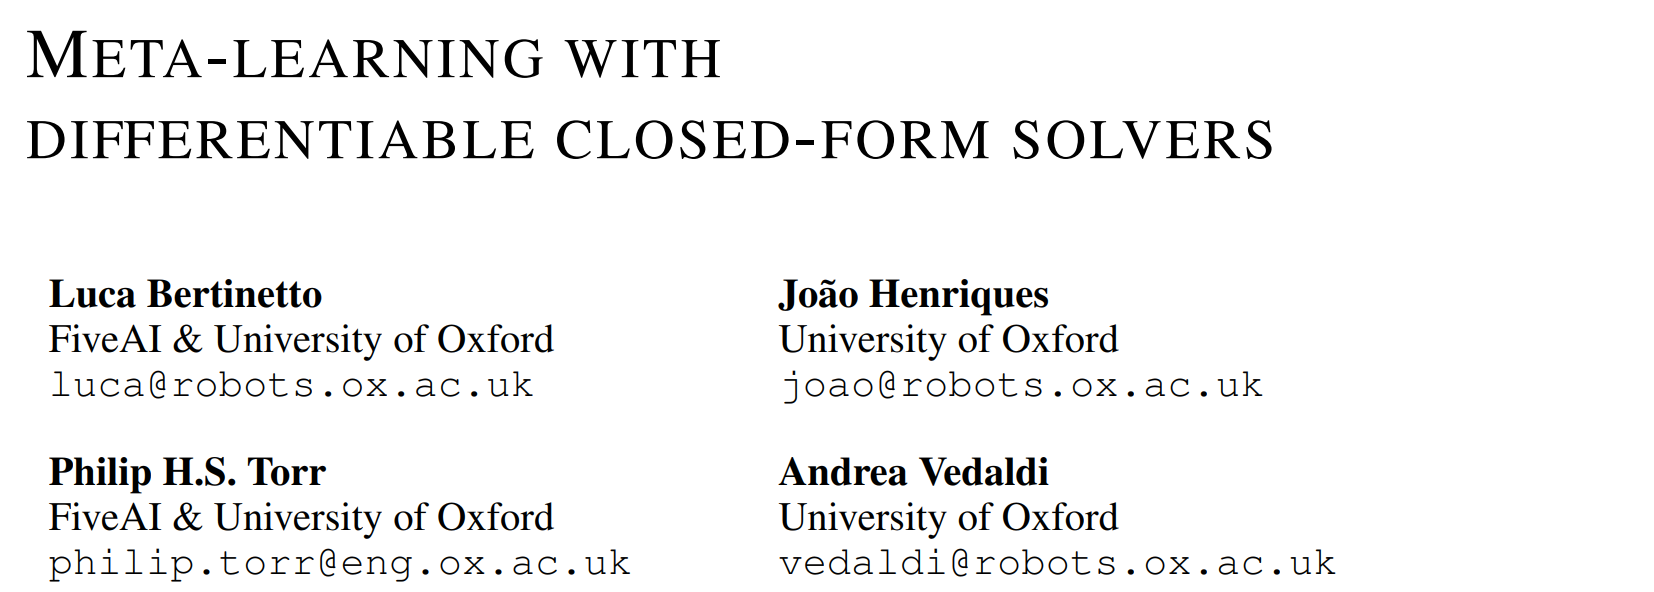
\includegraphics[width=\textwidth]{fig/r2d2-title.png}
  \center ICLR 2019
\end{frame}

\begin{frame}[t]{Motivation}
  Base learner $\mathcal{A}$:
  \begin{itemize}
    \item metric-based: nearest neighbor
    \item gradient-based: few-step GD
  \end{itemize}

  \pause
  \vspace{2cm}
  \center \LARGE{太弱了...}
\end{frame}

\begin{frame}[t]{Idea}
  Let $\mathcal{A}$ be ridge regression
\end{frame}

\begin{frame}[t]{Idea}
  Let $\mathcal{A}$ be ridge regression

  \vspace{1cm}
  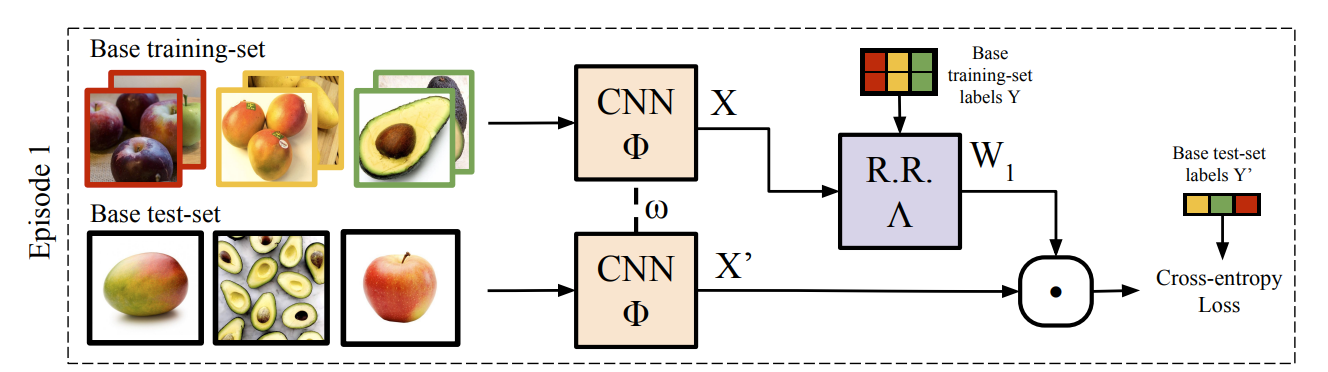
\includegraphics[width=\textwidth]{fig/r2d2.png}
\end{frame}

\begin{frame}[t]{Ridge Regression Base Learner (R2-D2)}
  In inner loop, only modify the last layer, denote the weight as $W \in \mathbb{R}^{e \times c}$

  \begin{equation*}
    \begin{aligned}
      W^\star &= \arg\min_W || XW-Y ||^2 + \lambda ||W||^2 \\
              &= (X^TX + \lambda I)^{-1} X^TY
    \end{aligned}
  \end{equation*}

  where $X \in \mathbb{R}^{N \times e}$, $Y \in \mathbb{R}^{N \times c}$ (stacked as rows)

  each row in $X$ is the embedding via feature encoder $\Phi$
\end{frame}

\begin{frame}[t]{Woodbury Formula applied to the closed-form solution}

  Since $X^T X \in  \mathbb{R}^{e \times e}$ is quadratical with dimension of embedding, \\
  it is time-consuming when calculating inverse

  \begin{equation*}
    \boxed{W^\star = X^T(X X^T + \lambda I)^{-1}Y}
  \end{equation*}

  Now $X X^T \in \mathbb{R}^{N \times N}$ (since \textbf{few-shot}, $N$ is small)
\end{frame}

\begin{frame}[t]{Results on miniImageNet \& CIFAR-FS}
  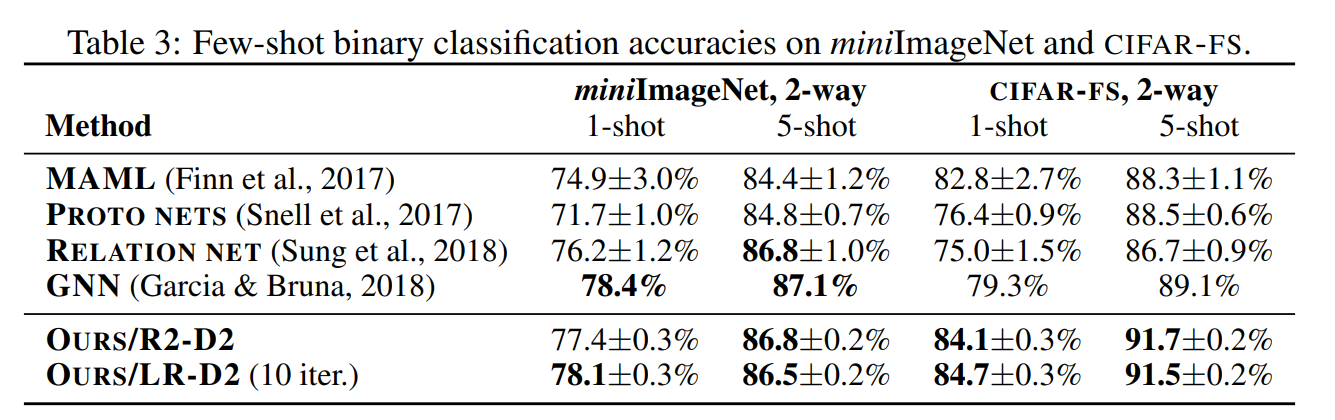
\includegraphics[width=\textwidth]{fig/r2d2-result.png}

  LR-D2: Logistic Regression solved with Newton method
\end{frame}

\begin{frame}[t]{R2-D2}
  \begin{itemize}
    \item More powerful base learner $\mathcal{A}$ to learn the last layer weight $W$
    \item Outer loop use GD to learn $\Phi$, $\lambda$
  \end{itemize}
\end{frame}

\begin{frame}{Conclusion}
  \begin{itemize}
    \item More powerful inner-loop optimization beyond few-step GD
    \item Regularization to make the outer-loop optimization computation faster
  \end{itemize}
\end{frame}
%\section{MISC}
\begin{frame}
	\begin{center}
    %\weib{\LARGE{謝謝聆聽!}}
    \LARGE{Questions?}
	\end{center}
\end{frame}

\end{document} 
